\newpage
\section{Suggested solutions: Fourier Transform}
\begin{enumerate}
\item Consider the rectangular signal 
$$x(t)=u(t+1)-u(t-1)$$

\begin{enumerate}[a)]
\item The signal $x(t)$ is a box of width $2$ with corners at $t=\pm 1$ and height $1$. 

\item Scaling the signal as $y(t)=x(2t)$ gives another rectangular box function. In this case the box starts and ends at $t=\pm 1/2$, so the width is $1$. Both of these signals are illustrated in Figure .

\begin{figure}
    \centering
    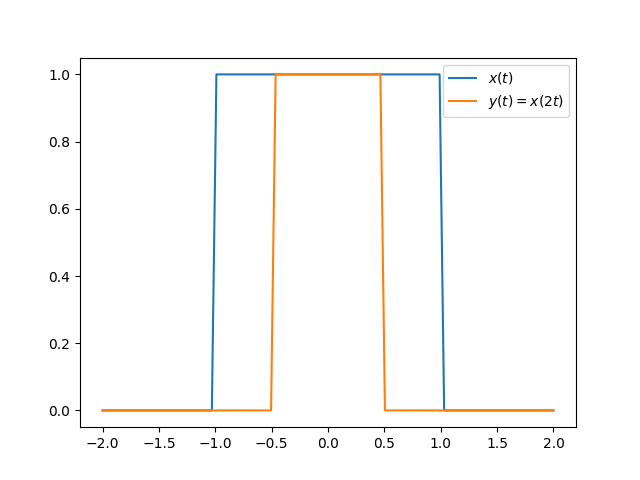
\includegraphics{ch08/figures/fig:ex8.1a.png}
    \caption{Drawing of signal $x(t)$ compared to $y(t)$}
    \label{fig:ex8.1a}
\end{figure}

\item The Fourier transforms for these signals are
\begin{align*}
    \hat{x}(\omega)&=\int_{-\infty}^{\infty}x(t)e^{-i\omega t}dt=\int_{-1}^{1}e^{-i\omega t}dt  \\
    &=-\frac{1}{i\omega}[e^{-i\omega t}]_{-1}^{1}=\frac{1}{i\omega}\left[e^{i\omega}-e^{-i\omega}\right]=\frac{2\sin(\omega)}{\omega}
\end{align*}
and for $y(t)$
\begin{align*}
    \hat{y}(\omega)&=\int_{-\infty}^{\infty}y(t)e^{-i\omega t}dt=\int_{-\frac{1}{2}}^{\frac{1}{2}}e^{-i\omega t}dt  \\
    &=-\frac{1}{i\omega}[e^{-i\omega t}]_{-\frac{1}{2}}^{\frac{1}{2}}=\frac{1}{i\omega}\left[e^{\frac{i}{2}\omega}-e^{-\frac{i}{2}\omega}\right]=\frac{2\sin(\omega/2)}{\omega}.
\end{align*}

\item For $\hat{x}(\omega)$ we have that the zeros occur for $\omega=n\pi$, giving a spacing of $1$ between the zeros. On the other hand, $\hat{y}(\omega)$ has its zeros occurring at $\omega=2n\pi$. In conclusion, $\hat{x}(\omega)$ has a spacing of $1$, while $\hat{y}(\omega)$ has a spacing of $2$. In this case \ref{eq:timescale_ft_pair} doesn't hold. The reason is due to the theorem relying on continuity and differentiability and this is not the case here. 
\end{enumerate}
\item
\begin{enumerate}[a)]
\item If 
$$x(t)=\delta(t+2)+\delta(t)+\delta(t-2)$$
then by linearity we have that
$$\hat{x}(\omega)=\mathcal{F}\{x(t)\}=\mathcal{F}\{\delta(t+2)\}+\mathcal{F}\{\delta(t)\}+\mathcal{F}\{\delta(t-2)\}$$
now, by using time shift properties we get
$$\hat{x}(\omega)=\mathcal{F}\{x(t)\}=\underline{\underline{e^{2i\omega}+1+e^{-2i\omega}}}$$
by Equation \ref{eq:fttss}.

\item Can rewrite the signal using the sinc function as
$$x(t)=\frac{\sin(100\pi(t-2))}{\pi(t-2)}=100\text{sinc}(100(t-2)).$$
Then by Equation \ref{eq:ft:timeshift} and Equation \ref{eq:ft:sinc} the Fourier transform is
$$\hat{x}(\omega)=100e^{-2i\omega}\mathcal{F}\{\text{sinc}100t\}=100e^{-2i\omega} \frac{1}{100}[u(\omega+100\pi)-u(\omega-100\pi)]$$
giving
$$\hat{x}(\omega)=\underline{\underline{e^{-2i\omega}[u(\omega+100\pi)-u(\omega-100\pi)]}}.$$

\item Take
$$x(t)=e^{-t}u(t)-e^{-t}u(t-4),$$
then by linearity the Fourier transform is
$$\hat{x}(\omega)=\mathcal{F}\{x(t)\}=\mathcal{F}\{e^{-t}u(t)\}-\mathcal{F}\{e^{-t}u(t-4)\}.$$
The last term can be simplified using the time shift property with $\tau=-4$ giving
$$\hat{x}(\omega)=\mathcal{F}\{e^{-t}u(t)\}-e^{-4i\omega}\mathcal{F}\{e^{-t}u(t)\}.$$
The Fourier transform of $e^{-t}u(t)$ is easily found as it is an exponential decay with $\beta=1$, hence
$$\hat{x}(\omega)=\frac{1}{1+i\omega}-e^{-4i\omega}\frac{1}{1+i\omega}=\underline{\underline{\frac{1}{1+i\omega}\left(1-e^{-4i\omega}\right)}}.$$
\end{enumerate}


\item
\begin{enumerate}[a)]
\item Let $\hat{x}(\omega)=2+\cos\omega$, then the inverse Fourier transform is
\begin{align*}
    x(t)&=\mathcal{F}^{-1}\{\hat{x}(\omega)\}=\mathcal{F}^{-1}\{2\}+\mathcal{F}^{-1}\{\cos\omega\} \\
    &=2\delta(t)+\frac{1}{2}(\mathcal{F}^{-1}\{e^{i\omega}\}+\mathcal{F}^{-1}\{e^{-i\omega})\} \\ &=\underline{\underline{2\delta(t)+\frac{1}{2}(\delta(t+1)+\delta(t-1))}}
\end{align*}
as $\mathcal{F}^{-1}\{e^{i\omega\tau}\}=\delta(t+\tau)$.

\item For $\hat{x}(\omega)=\frac{1}{1+i\omega}-\frac{1}{2+i\omega}$, then the inverse Fourier transform is
\begin{align*}
    x(t)&=\mathcal{F}^{-1}\{\hat{x}(\omega)\}=\mathcal{F}^{-1}\left\{\frac{1}{1+i\omega}\right\}-\mathcal{F}^{-1}\left\{\frac{1}{2+i\omega}\right\} \\
    &=\underline{\underline{e^{-t}u(t)-e^{-2t}u(t)}},
\end{align*}
as $\mathcal{F}\{e^{-\beta t}u(t)\}=\frac{1}{\beta+i\omega}$. 

\item Let $\hat{x}(\omega)=i\delta(\omega-100\pi)-i\delta(\omega+100\pi)$, then the inverse Fourier transform is
\begin{align*}
    x(t)&=\mathcal{F}^{-1}\{\hat{x}(\omega)\}=i\mathcal{F}^{-1}\{\delta(\omega-100\pi)\}-i\mathcal{F}^{-1}\{\delta(\omega+100\pi)\} \\
    &=\frac{i}{2\pi}e^{100\pi it}-\frac{i}{2\pi}e^{-100\pi it} \\
    &=\frac{1}{2\pi}(e^{i\pi/2}e^{100\pi i t}+e^{-i\pi/2}e^{-100\pi i t}) \\
    &=\underline{\underline{\frac{1}{\pi}\cos\left(100\pi t+\frac{\pi}{2}\right)}}.
\end{align*}
\end{enumerate}

\item   
\begin{enumerate}[a)]
\item Let $x(t)=u(t+3)u(3-t)$, then $x(t)$ is a rectangular function with corners at $t=\pm 3$ and height $1$. Therefore we have 
$$\hat{x}(\omega)=\mathcal{F}\{x(t)\}=\int_{-\infty}^{\infty}u(t+3)u(3-t)e^{-i\omega t}dt=\int_{-3}^{3}e^{-i\omega t}dt=\left[\frac{1}{-i\omega}e^{-i\omega t}\right]_{t=-3}^{3}.$$
Evaluating this yields
$$\hat{x}(\omega)=-\frac{1}{i\omega}(e^{-3i\omega}-e^{3i\omega})=\frac{1}{i\omega}(e^{3i\omega}-e^{-3i\omega})=\underline{\underline{\frac{2\sin(3\omega)}{\omega}}}.$$

\item Consider the signal $x(t)$ given as
$$x(t)=\sin(4\pi t)\sin(50\pi t),$$
then 
\begin{align*}
    \sin(4\pi t)&=\frac{1}{2i}(e^{4\pi i t}-e^{-4\pi it}), \\
    \sin(50\pi t)&=\frac{1}{2i}(e^{50\pi it}-e^{-50\pi it}),
\end{align*}
which gives
$$x(t)=\frac{1}{2i}\left(e^{4\pi it}-e^{-4\pi it}\right)\frac{1}{2i}\left(e^{50\pi it}-e^{-50\pi it}\right)=-\frac{1}{4}\left(e^{i54\pi t}-e^{-i46\pi t}-e^{i46\pi t}+e^{-i54\pi t}\right),$$
Next, we evaluate the transform
$$\hat{x}(\omega)=\int_{-\infty}^{\infty}x(t)e^{-i\omega t}dt=-\frac{1}{4}\int_{-\infty}^{\infty}\left(e^{i54\pi t}-e^{-i46\pi t}-e^{i46\pi t}+e^{-i54\pi t}\right)e^{-i\omega t}dt,$$
and obtain
$$\hat{x}(\omega)=\underline{\underline{-\frac{\pi}{2}[\delta(\omega-54\pi)-\delta(\omega+46\pi)-\delta(\omega-46\pi)+\delta(\omega+54\pi)]}}.$$

\item Let
$$x(t)=\frac{\sin(4\pi t)}{\pi t}\sin(50\pi t)$$
then to compute the Fourier transform we apply the convolution theorem, have that
\begin{align*}
    \mathcal{F}\left\{\frac{\sin(4\pi t)}{\pi t}\right\}&=[u(\omega+4\pi)-u(\omega-4\pi)]=\hat{x}_{1}(\omega) \\
    \mathcal{F}\left\{\sin(50\pi t)\right\}&=-i\pi[\delta(\omega-50\pi)-\delta(\omega+50\pi)]=\hat{x}_{2}(\omega)
\end{align*}
then in frequency domain we get
\begin{align*}
\hat{x}_{1}(\omega)*\hat{x}_{2}(\omega)&=\frac{1}{2\pi}\int_{-\infty}^{\infty}\hat{x}_{1}(\tau)\hat{x}_{2}(\omega-\tau)d\tau \\
&=\frac{1}{2\pi}\int_{-\infty}^{\infty}[u(\tau+4\pi)-u(\tau-4\pi)][-\pi i(\delta(\omega-\tau-50\pi)-\delta(\omega-\tau+50\pi))]d\tau \\
&=\frac{1}{2i}\int_{-\infty}^{\infty}[u(\tau+4\pi)-u(\tau-4\pi)][\delta((\omega-50\pi)-\tau)-\delta((\omega+50\pi)-\tau)]d\tau
\end{align*}
The integral consists of four terms, these being
\begin{align*}
    \int_{-\infty}^{\infty}u(\tau+4\pi)\delta(\omega-50\pi-\tau)d\tau&=u(\omega-50\pi+4\pi)=u(\omega-46\pi) \\
    \int_{-\infty}^{\infty}u(\tau+4\pi)\delta(\omega+50\pi-\tau)d\tau&=u(\omega+50\pi+4\pi)=u(\omega+54\pi) \\
    \int_{-\infty}^{\infty}u(\tau-4\pi)\delta(\omega-50\pi-\tau)d\tau&=u(\omega-50\pi-4\pi)=u(\omega-54\pi) \\
    \int_{-\infty}^{\infty}u(\tau-4\pi)\delta(\omega+50\pi-\tau)d\tau&=u(\omega+50\pi-4\pi)=u(\omega+46\pi)
\end{align*}
combining all these we get
$$\hat{x}(\omega)=\underline{\underline{\frac{1}{2i}[u(\omega-46\pi)-u(\omega+54\pi)-u(\omega-54\pi)+u(\omega+46\pi)]}}.$$

\item If $\hat{x}(\omega)=\cos^{2}(\omega)$, then we find $x(t)$ by using the inverse Fourier transform
$$x(t)=\frac{1}{2\pi}\int_{-\infty}^{\infty}\cos^{2}(\omega)e^{i\omega t}d\omega.$$
Firstly, we rewrite our function as
$$\cos^{2}(\omega)=\left(\frac{1}{2}\left(e^{i\omega}+e^{-i\omega}\right)\right)^{2}=\frac{1}{4}\left(e^{2i\omega }+e^{-2i\omega}+2\right)$$
Substituting this we obtain
$$x(t)=\frac{1}{2\pi}\int_{-\infty}^{\infty}\frac{1}{4}\left(e^{2i\omega }+e^{-2i\omega}+2\right)e^{i\omega t}d\omega=\underline{\underline{\frac{1}{8\pi}[\delta(t+2)+2\delta(t)+\delta(t-2)]}}.$$
\end{enumerate}

\item Let $\hat{x}(\omega)$ be the Fourier transform of $x(t)$. Define $y(t)=x(t-\tau)$, then the Fourier transform of $y(t)$ is by definition
$$\hat{y}(\omega)=\int_{-\infty}^{\infty}y(t)e^{-i\omega t}dt=\int_{-\infty}^{\infty}x(t-\tau)e^{-i\omega t}dt.$$
Let $u=t-\tau$, then $du=dt$, thus
$$\hat{y}(\omega)=\int_{-\infty}^{\infty}x(u)e^{-i\omega(u+\tau)}du=e^{-i\omega\tau}\int_{-\infty}^{\infty}x(u)e^{-i\omega u}du=e^{-i\omega u}\hat{x}(\omega),$$
as $\hat{x}(\omega)=\int_{-\infty}^{\infty}x(t)e^{-i\omega t}dt$. 




\end{enumerate}